\documentclass{beamer}

\setbeamertemplate{navigation symbols}{}
\setbeamertemplate{theorems}[numbered]
\setbeamertemplate{items}[default]
\setbeamercovered{dynamic}
\setlength{\unitlength}{1cm}
\setbeamertemplate{footline}[frame number]

\usepackage{setspace}
\usepackage{polski}
\usepackage{graphicx}
\usepackage{mathtools} 
\usepackage{tikz}
\usetikzlibrary{arrows,automata,snakes,positioning,calc}
\DeclareMathOperator{\rank}{rank}
\usetheme{Frankfurt}
\usecolortheme{seahorse} %crane
\useinnertheme{circles}
\usepackage{subfigure}
\usepackage{subcaption}
\usepackage{float}
%\pgfpagesuselayout{4 on 1 with notes}[a4paper,border shrink=3mm]


\title{Mechanizm multilateracji w rozproszonej sieci sensorów audio}

\author{
	\textbf{Gabriel Budziński}
	\newline \newline
	Praca napisana pod kierunkiem \textbf{dra inż. Przemysława Błaśkiewicza}
}

\begin{document}

\begin{frame}[plain]{}
	\titlepage
\end{frame}

\section{Multilateracja}
\begin{frame}
    \begin{block}{Multiateracja}
        Weźmy punkt $(x, y) \in \mathbb{R}^2$ i oznaczmy go $N$, ponadto weźmy zbiór $n$ punktów $\left\{(x_i, y_i): i \in [n]\right\} \subset \mathbb{R}^2$, który oznaczmy $\mathcal{O}$, a punkty należące do zbioru odpowiednio $O_i$. Niech $d_i$ będzie odległością $d(N, O_i)$. Znając współrzędne punktów $O_i$ oraz odległości $d_i$ chcemy znaleźć $(x, y)$.
        % \begin{equation}
        %     \begin{dcases}
        %         {(x - x_1)}^2 + {(y - y_1)}^2 = {d_1}^2 \\
        %         {(x - x_2)}^2 + {(y - y_2)}^2 = {d_2}^2 \\
        %         {(x - x_n)}^2 + {(y - y_n)}^2 = {d_n}^2\,.
        %     \end{dcases}
        % \end{equation}
    \end{block}
    \begin{figure}[!h]
        \begin{tikzpicture}[scale=0.80]
            \coordinate (O1) at (0,0);
            \coordinate (O2) at (6,0);
            \coordinate (O3) at (6,6);
            \coordinate (O4) at (0,6);
            \coordinate (N) at (0.75,4.5);
            \filldraw[black] (O1) circle (2pt) node[left]{$O_1$};
            \filldraw[black] (O2) circle (2pt) node[right]{$O_2$};
            \filldraw[black] (O3) circle (2pt) node[right]{$O_3$};
            \filldraw[black] (N) circle (2pt) node[above left]{$N$};
            \draw[black] (O1) -- node[right]{$d_1$} (N);
            \draw[black] (O2) -- node[left]{$d_2$} (N);
            \draw[black] (O3) -- node[above]{$d_3$} (N);
            \draw[loosely dashed, thin] (O1) -- (O2);
            \draw[loosely dashed, thin] (O2) -- (O3);
            \draw[loosely dashed, thin] (O3) -- (O4);
            \draw[loosely dashed, thin] (O4) -- (O1);
        \end{tikzpicture}
    \end{figure}
\end{frame}
\begin{frame}
    \begin{block}{Postać wyjściowa}
        \begin{equation*}
            \begin{dcases}
                {(x - x_1)}^2 + {(y - y_1)}^2 = {d_1}^2 \\
                {(x - x_2)}^2 + {(y - y_2)}^2 = {d_2}^2 \\
                \mspace{110mu}\vdots                    \\
                {(x - x_n)}^2 + {(y - y_n)}^2 = {d_n}^2
            \end{dcases}
        \end{equation*}
    \end{block}

    \begin{block}{Obrane przekształcenie}
        \begin{equation*}
            \left[
                \begin{matrix}
                    1 & -2x_1 & -2y_1  \\
                    1 & -2x_2 & -2y_2  \\
                    \multicolumn{3}{c}{\vdots} \\
                    1 & -2x_n & -2y_n \\
                \end{matrix}
                \right]
            \left[
                \begin{matrix}
                    x^2 + y^2 \\
                    x         \\
                    y         \\
                \end{matrix}
                \right]
            =
            \left[
                \begin{matrix}
                    d_1^2 - x_1^2 - y_1^2 \\
                    d_2^2 - x_2^2 - y_2^2 \\
                    \vdots                \\
                    d_n^2 - x_n^2 - y_n^2 \\
                \end{matrix}
                \right]
        \end{equation*}
        \begin{equation*}
            \mathbf{A} \cdot \mathbf{x} = \mathbf{b}
        \end{equation*}
    \end{block}
\end{frame}
\begin{frame}
    \begin{block}{Rozwiązanie}
        Obrano rozwiązanie aproksymacyjne w sensie najmniejszych kwadratów:
        \begin{equation*}
            \sum_{i=1}^{n}{\left|\sum_{j=1}^{m}{A_{ij}x_j} - b_i\right|^2} = ||\mathbf{A}\hat{\mathbf{x}} - \mathbf{b}||^2\,,
        \end{equation*}
        które otrzymujemy poprzez rozwiązanie równania normalnego
        \begin{equation*}
            \mathbf{A}^T\mathbf{A}\hat{\mathbf{x}} = \mathbf{A}^T\mathbf{b}
        \end{equation*}
    \end{block}

    % \begin{block}{Istnienie rozwiązania}
    %     Zakładając, że żadna trójka odbiorników nie jest współliniowa ($\rank\mathbf{A} = m$), co daje odwracalność $\mathbf{A}$ i istnienie $\hat{\mathbf{x}}$.
    % \end{block}
\end{frame}
\section{Synchronizacja czasu}
\begin{frame}
    \begin{block}{Metody synchronizacji}
        \begin{itemize}
            \item Synchronizacja programowa
                \begin{itemize}
                    \item Synchronizacja NTP
                    \item Synchronizacja pomiaru przesunięć
                \end{itemize}
            \item Synchronizacja sprzętowa
                \begin{itemize}
                    \item Synchronizacja mikrofonowa
                \end{itemize}
        \end{itemize}
    \end{block}
    \begin{figure}[H]
        \centering
        \resizebox{0.7\textwidth}{!}{%
            \begin{tikzpicture}
                \tikzstyle{every node}=[font=\Huge]
                \draw [line width=1pt] (10,24.25) -- (36.25,24.25);
                \draw [line width=1pt] (10,15.5) -- (36.25,15.5);
                \draw [line width=1pt, ->] (12.5,15.5) -- (18.75,24.25);
                \draw [line width=1pt, ->] (27.5,24.25) -- (33.75,15.5);
                \draw [line width=1pt] (20,15.5) -- (20,21.75);
                \draw [line width=1pt] (26.25,24.25) -- (26.25,18);
                \draw [line width=1pt, <->] (20,19.75) -- (26.25,19.75)node[pos=0.5, fill=white]{$\theta$};
                \node [font=\Huge] at (12.5,14.75) {$T_{i-3}$};
                \node [font=\Huge] at (18.75,25) {$T_{i-2}$};
                \node [font=\Huge] at (27.5,24.75) {$T_{i-1}$};
                \node [font=\Huge] at (34,14.75) {$T_i$};
                \node [font=\Huge] at (23,24.75) {$B$};
                \node [font=\Huge] at (23,14.75) {$A$};
            \end{tikzpicture}
        }%
    \end{figure}
\end{frame}
\begin{frame}
    \begin{block}{Synchronizacja NTP}
        \begin{figure}[H]
            \centering
            \resizebox{0.7\textwidth}{!}{%
                \begin{tikzpicture}
                    \tikzstyle{every node}=[font=\Huge]
                    \draw [line width=1pt] (10,24.25) -- (36.25,24.25);
                    \draw [line width=1pt] (10,15.5) -- (36.25,15.5);
                    \draw [line width=1pt, ->] (12.5,15.5) -- (18.75,24.25);
                    \draw [line width=1pt, ->] (27.5,24.25) -- (33.75,15.5);
                    \draw [line width=1pt] (20,15.5) -- (20,21.75);
                    \draw [line width=1pt] (26.25,24.25) -- (26.25,18);
                    \draw [line width=1pt, <->] (20,19.75) -- (26.25,19.75)node[pos=0.5, fill=white]{$\theta$};
                    \node [font=\Huge] at (12.5,14.75) {$T_{i-3}$};
                    \node [font=\Huge] at (18.75,25) {$T_{i-2}$};
                    \node [font=\Huge] at (27.5,24.75) {$T_{i-1}$};
                    \node [font=\Huge] at (34,14.75) {$T_i$};
                    \node [font=\Huge] at (23,24.75) {$B$};
                    \node [font=\Huge] at (23,14.75) {$A$};
                \end{tikzpicture}
            }%
        \end{figure}
        $a = T_{i-2} - T_{i-3}$, $b = T_{i-1} - T_i$, $\delta_i = a - b$, $ \theta_i = \frac{a+b}{2}$
        \[\theta_i - \frac{\delta_i}{2} \leqslant \theta \leqslant \theta_i + \frac{\delta_i}{2}.\]
    \end{block}
\end{frame}

\begin{frame}
    \begin{block}{Synchronizacja pomiaru przesunięć}
        Węzeł wysyła $n$ wiadomości zawierających aktualną wartość zegara, która po odebraniu przez serwer jest porównywana z zegarem w nim dostępnym.
    \end{block}
    \begin{block}{Synchronizacja mikrofonowa}
        Nadajnik umieszczany jest w odległości $0$ od odbiornika. Nadajemy $n$ sygnałów dźwiękowych i porównujemy czas nadania i odbioru.
    \end{block}
\end{frame}
\begin{frame}
    \begin{block}{Synchronizacja NTP}
        Pomiary wybranych odległości w przedziale $[0,1]$. Wykres po lewej - dane przed normalizacją do punktu $0$, natomiast prawy po normalizacji, okrojony do interesującego przedziału. Prosta $y=x$ wskazuje oczekiwane wyniki. Na prawym wykresie dodatkowa prosta przedstawia przybliżony współczynnik skalowania odległości.
    \end{block}
    \begin{figure}
        \centering
        \includegraphics[width=0.49\textwidth]{../pics/ntp_sync_dist/dists.png}
        \includegraphics[width=0.49\textwidth]{../pics/ntp_sync_dist/dists_close.png}
    \end{figure}
\end{frame}
\begin{frame}
    \begin{block}{Synchronizacja pomiaru przesunięć}
        Pomiary wybranych odległości w przedziale $[0,1]$. Wykres po lewej - dane przed normalizacją do punktu $0$, natomiast prawy po normalizacji, okrojony do interesującego przedziału. Prosta $y=x$ wskazuje oczekiwane wyniki. Na prawym wykresie dodatkowa prosta przedstawia przybliżony współczynnik skalowania odległości.
    \end{block}
    \begin{figure}
        \centering
        \includegraphics[width=0.49\textwidth]{../pics/time_deltas_dist/dists.png}
        \includegraphics[width=0.49\textwidth]{../pics/time_deltas_dist/dists_close.png}
    \end{figure}
\end{frame}
\begin{frame}
    \begin{figure}
        \centering
        \includegraphics[width=0.49\textwidth]{../pics/mic_sync_dist/dists.png}
        \includegraphics[width=0.49\textwidth]{../pics/mic_sync_dist/dists_close.png}
        \caption{synchronizacja mikrofonowa}
    \end{figure}
\end{frame}
\begin{frame}
    % \begin{figure}
    %     \centering
        % \begin{subfigure}{}
        %     \centering
            \includegraphics[width=0.49\textwidth]{../pics/mic_sync_dist/dists_close_long_0_mean.png}
        %     \caption{pomiar 1.}
        % \end{subfigure}%
        % \begin{subfigure}{}
        %     \centering
            \includegraphics[width=0.49\textwidth]{../pics/mic_sync_dist/dists_close_long_1_mean.png}
        %     \caption{pomiar 2.}
        % \end{subfigure}
        % \begin{subfigure}{0.5\textwidth}
        %     \centering
            \includegraphics[width=0.49\textwidth]{../pics/mic_sync_dist/dists_close_long_2_mean.png}
            % \caption{pomiar 3.}
        % \end{subfigure}%
        % \begin{subfigure}{0.5\textwidth}
        %     \centering
            \includegraphics[width=0.49\textwidth]{../pics/mic_sync_dist/dists_close_long_3_mean.png}
            % \caption{pomiar 4.}
        % \end{subfigure}
        % \caption{Średnie obliczonych odległości}
    % \end{figure}
\end{frame}
\section{Ewaluacja działania}
\begin{frame}
    \begin{figure}[H]
        \centering
        \resizebox{\textwidth}{!}{%
            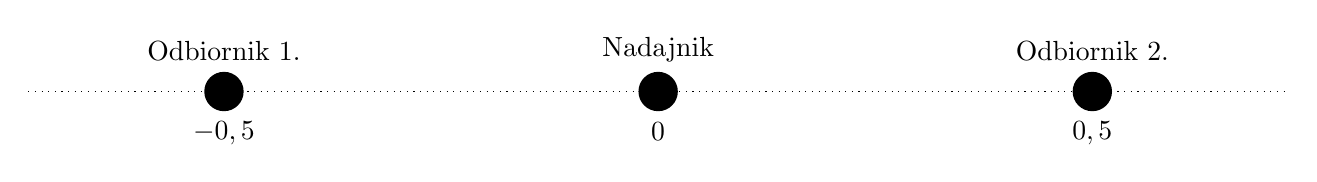
\begin{tikzpicture}[pointnode/.style={circle, fill=black}, node distance=5cm, minimum size=5mm]
                \node[pointnode,
                label=above:{Nadajnik},
                label=below:{$0$}] (N) {};
                \node[pointnode,
                label=above:{Odbiornik 1.},
                label=below:{$-0,5$}] (O1) [left=of N] {};
                \node[pointnode,
                label=above:{Odbiornik 2.},
                label=below:{$0,5$}] (O2) [right=of N] {};
                \draw[-, thin, dotted] (-8,0) -- (8,0);
            \end{tikzpicture}
        }%
    \end{figure}
    \begin{figure}
        \centering
        \includegraphics[width=\linewidth]{../pics/mult_lat_1d/position_[0.25]_2.png}
        \caption{Punkt w pozycji (0,25), 2 mikrofony}
    \end{figure}
\end{frame}
\begin{frame}{}
    \begin{figure}
        \centering
        \begin{subfigure}{}
            \centering
            \includegraphics[width=0.6\linewidth]{../pics/mult_lat_1d/positions_2_mean.png}
            \caption{2 mikrofony}
        \end{subfigure}%
        \begin{subfigure}{}
            \centering
            \includegraphics[width=0.6\linewidth]{../pics/mult_lat_1d/positions_4_mean.png}
            \caption{4 mikrofony}
        \end{subfigure}
    \end{figure}
\end{frame}
\begin{frame}{}
    \begin{columns}
        \begin{column}{0.5\textwidth}
            \begin{figure}
                \centering
                \includegraphics[width=\textwidth]{../pics/mult_lat_2d_angle/positions_0_mean.png}
                \caption{rotacja $0^{\circ}$}
            \end{figure}
        \end{column}
        \begin{column}{0.5\textwidth}
            \begin{figure}
                \centering
                \includegraphics[width=\textwidth]{../pics/mult_lat_2d_angle/positions_45_mean.png}
                \caption{rotacja $45^{\circ}$}
            \end{figure}
        \end{column}
    \end{columns}
\end{frame}

\begin{frame}
    \begin{figure}
        \centering
        \includegraphics[width=0.5\textwidth]{../pics/mult_lat_2d_angle/positions_90_mean.png}
        \caption{rotacja $90^{\circ}$}
    \end{figure}
\end{frame}
\begin{frame}{}
    \frametitle{Wpływ liczby odbiorników}
    \begin{columns}
        \begin{column}{0.5\textwidth}
            \begin{figure}
                \centering
                \includegraphics[width=\textwidth]{../pics/mult_lat_2d_num/positions_3_mean.png}
                \caption{3 mikrofony}
            \end{figure}
        \end{column}
        \begin{column}{0.5\textwidth}
            \begin{figure}
                \centering
                \includegraphics[width=\textwidth]{../pics/mult_lat_2d_num/positions_4_mean.png}
                \caption{4 mikrofony}
            \end{figure}
        \end{column}
    \end{columns}
\end{frame}

\begin{frame}{}
    \frametitle{Wpływ liczby odbiorników}
    \begin{columns}
        \begin{column}{0.5\textwidth}
            \begin{figure}
                \centering
                \includegraphics[width=\textwidth]{../pics/mult_lat_2d_num/positions_5_mean.png}
                \caption{5 mikrofonów}
            \end{figure}
        \end{column}
        \begin{column}{0.5\textwidth}
            \begin{figure}
                \centering
                \includegraphics[width=\textwidth]{../pics/mult_lat_2d_num/positions_6_mean.png}
                \caption{6 mikrofonów}
            \end{figure}
        \end{column}
    \end{columns}
\end{frame}

\begin{frame}{}
    \frametitle{Wpływ liczby odbiorników}
    \begin{columns}
        \begin{column}{0.5\textwidth}
            \begin{figure}
                \centering
                \includegraphics[width=\textwidth]{../pics/mult_lat_2d_num/positions_7_mean.png}
                \caption{7 mikrofonów}
            \end{figure}
        \end{column}
        \begin{column}{0.5\textwidth}
            \begin{figure}
                \centering
                \includegraphics[width=\textwidth]{../pics/mult_lat_2d_num/positions_8_mean.png}
                \caption{8 mikrofonów}
            \end{figure}
        \end{column}
    \end{columns}
\end{frame}
\begin{frame}
    \begin{block}{Wnioski}
        Czynniki wpływające na jakość pomiarów:
        \begin{itemize}
            \item zmienne własności akustyczne otoczenia,
            \item czułość wzmacniaczy operacyjnych mikrofonów,
            \item liczba odbiorników.
        \end{itemize}
        Dalsze kroki rozwoju systemu:
        \begin{itemize}
            \item poprawa tolerancji błędnych odczytów odległości,
            \item dokładniejsze przebadanie funkcji korekcyjnej.
        \end{itemize}
    \end{block}
\end{frame}
\appendix
\begin{frame}
\begin{center}
	Dziękuję za uwagę.
\end{center}
\end{frame}

\end{document}